%%%%%%%%%%%%%%%%%%%%%%%%%%%%%%%%%%%%%
%
%file name = latextop.tex
%
%LATEXTOP TEX%%%%%%%%%%%%%%%%%%%%%%%%%%
%\documentclass[12pt, a4j, landscape]{jarticle}
\documentclass[12pt]{article}
\usepackage[dvips]{epsfig}
\usepackage{amsthm,amsmath,amssymb}
%\usepackage{ascmac}
%\usepackage{latexsym}
\usepackage{latexsym}
% \usepackage{times}
%\usepackage[dvipdfmx]{graphicx}
\usepackage{graphics}
\usepackage{url}
\usepackage{placeins}
\usepackage{hyperref}
\usepackage{color}
\usepackage{bm}
\usepackage{comment}
\usepackage{statex}


\setlength{\evensidemargin}{0cm}
\setlength{\oddsidemargin}{0cm}
%\setlength{\textwidth}{26cm}
%\setlength{\textheight}{18cm}
%\setlength{\textwidth}{6.25in}
\setlength{\textwidth}{6.45in}
%\setlength{\textheight}{8.5in}
\setlength{\textheight}{9.2in}
% \setlength{\topmargin}{-1.8cm}
% \setlength{\topmargin}{-1.0cm}
\setlength{\topmargin}{0in}
\setlength{\headheight}{0in}
\setlength{\headsep}{0in}
\setlength{\topskip}{0in} 


%%%%% Definition of Color ---> %%%%%
\def\TWhite{\textcolor{white}}
\def\TBlack{\textcolor{black}}
\def\TGray{\textcolor{gray}}
\def\TBlue{\textcolor{blue}}
\def\TGreen{\textcolor{green}}
\def\TYellow{\textcolor{yellow}}
\def\TRed{\textcolor{red}}
\def\TOrange{\textcolor{orange}}
\def\TViolet{\textcolor{violet}}
\def\TPurple{\textcolor{purple}} 
\def\TBrown{\textcolor{brown}}

\definecolor{blue}{rgb}{0,0,0.9}
\definecolor{red}{rgb}{0.9,0,0}
\definecolor{green}{rgb}{0,0.9,0}
\definecolor{violet}{rgb}{0.5804,0.0000,0.8275}  
\newcommand{\blue}[1]{\begin{color}{blue}#1\end{color}}
\newcommand{\magenta}[1]{\begin{color}{magenta}#1\end{color}}
\newcommand{\red}[1]{\begin{color}{red}#1\end{color}}
\newcommand{\green}[1]{\begin{color}{green}#1\end{color}}
\newcommand{\violet}[1]{\begin{color}{violet}#1\end{color}}
%%%%% <--- Definition of Color %%%%%


\def\@themcountersep{}
\def\thesection{\arabic{section}}

\newtheorem{THEO}{Theorem}[section]
\newtheorem{ALGo}[THEO]{Algorithm}
\newtheorem{CONJ}[THEO]{Conjecture}
\newtheorem{COND}[THEO]{Condition}
\newtheorem{CORO}[THEO]{Corollary}
\newtheorem{DEFI}[THEO]{Definition}
\newtheorem{EXAMP}[THEO]{Example}
\newtheorem{FACT}[THEO]{Fact}
\newtheorem{HYPO}[THEO]{Hypothesis}
\newtheorem{LEMM}[THEO]{Lemma}
\newtheorem{PROB}[THEO]{Problem}
\newtheorem{PROP}[THEO]{Proposition}
\newtheorem{REMA}[THEO]{Remark}
\newcommand{\theo}{\begin{THEO}}
\newcommand{\algo}{\begin{ALGo} \rm}
\newcommand{\cond}{\begin{COND}}
\newcommand{\conj}{\begin{CONJ}}
\newcommand{\coro}{\begin{CORO}}
\newcommand{\defi}{\begin{DEFI} \rm}
\newcommand{\examp}{\begin{EXAMP} \rm}
\newcommand{\fact}{\begin{FACT}}
\newcommand{\hypo}{\begin{HYPO} \rm}
\newcommand{\lemm}{\begin{LEMM}}
\newcommand{\prob}{\begin{PROB} \rm}
\newcommand{\prop}{\begin{PROP}}
\newcommand{\rema}{\begin{REMA} \rm}
\newcommand{\etheo}{\end{THEO}}
\newcommand{\ealgo}{\end{ALGo}}
\newcommand{\econd}{\end{COND}}
\newcommand{\econj}{\end{CONJ}}
\newcommand{\ecoro}{\end{CORO}}
\newcommand{\edefi}{\end{DEFI}}
\newcommand{\eexamp}{\end{EXAMP}}
\newcommand{\efact}{\end{FACT}}
\newcommand{\ehypo}{\end{HYPO}}
\newcommand{\elemm}{\end{LEMM}}
\newcommand{\eprob}{\end{PROB}}
\newcommand{\eprop}{\end{PROP}}
\newcommand{\erema}{\end{REMA}}
\def\br{\hfill\break}
\def\mAth{\mathsurround=0pt}
\def\eqalign#1{\,\vcenter{\openup1\jot \mAth
   \ialign{\strut\hfil$\displaystyle{##}$&$\displaystyle{{}##}$\hfil
     \crcr#1\crcr}}\,}

%
%file name = bflatex.tex
%
\def\0{\mbox{\bf 0}}
\def\1{\mbox{\bf 1}}
\def\2{\mbox{\bf 2}}
\def\3{\mbox{\bf 3}}
\def\4{\mbox{\bf 4}}
\def\5{\mbox{\bf 5}}
\def\6{\mbox{\bf 6}}
\def\7{\mbox{\bf 7}}
\def\8{\mbox{\bf 8}}
\def\9{\mbox{\bf 9}}
\def\a{\mbox{\boldmath $a$}}
\def\b{\mbox{\boldmath $b$}}
%\def\c{\mbox{\boldmath $c$}}
\def\cc{\mbox{\boldmath $c$}}
\def\d{\mbox{\boldmath $d$}}
\def\e{\mbox{\boldmath $e$}}
\def\f{\mbox{\boldmath $f$}}
\def\g{\mbox{\boldmath $g$}}
\def\h{\mbox{\boldmath $h$}}
\def\i{\mbox{\boldmath $i$}}
\def\j{\mbox{\boldmath $j$}}
\def\k{\mbox{\boldmath $k$}}
\def\l{\mbox{\boldmath $l$}}
\def\m{\mbox{\boldmath $m$}}
\def\n{\mbox{\boldmath $n$}}
\def\o{\mbox{\boldmath $o$}}
\def\p{\mbox{\boldmath $p$}}
\def\q{\mbox{\boldmath $q$}}
\def\r{\mbox{\boldmath $r$}}
\def\s{\mbox{\boldmath $s$}}
\def\t{\mbox{\boldmath $t$}}
\def\u{\mbox{\boldmath $u$}}
\def\v{\mbox{\boldmath $v$}}
\def\w{\mbox{\boldmath $w$}}
\def\x{\mbox{\boldmath $x$}}
\def\y{\mbox{\boldmath $y$}}
\def\z{\mbox{\boldmath $z$}}
\def\A{\mbox{\boldmath $A$}}
\def\B{\mbox{\boldmath $B$}}
\def\C{\mbox{\boldmath $C$}}
\def\D{\mbox{\boldmath $D$}}
\def\E{\mbox{\boldmath $E$}}
\def\F{\mbox{\boldmath $F$}}
\def\G{\mbox{\boldmath $G$}}
\def\H{\mbox{\boldmath $H$}}
\def\I{\mbox{\boldmath $I$}}
\def\J{\mbox{\boldmath $J$}}
\def\K{\mbox{\boldmath $K$}}
\def\L{\mbox{\boldmath $L$}}
\def\M{\mbox{\boldmath $M$}}
\def\N{\mbox{\boldmath $N$}}
\def\O{\mbox{\boldmath $O$}}
\def\P{\mbox{\boldmath $P$}}
\def\Q{\mbox{\boldmath $Q$}}
\def\R{\mbox{\boldmath $R$}}
\def\S{\mbox{\boldmath $S$}}
\def\T{\mbox{\boldmath $T$}}
\def\U{\mbox{\boldmath $U$}}
\def\V{\mbox{\boldmath $V$}}
\def\W{\mbox{\boldmath $W$}}
\def\X{\mbox{\boldmath $X$}}
\def\Y{\mbox{\boldmath $Y$}}
\def\Z{\mbox{\boldmath $Z$}}
\def\AC{\mbox{$\cal A$}}
\def\BC{\mbox{$\cal B$}}
\def\CC{\mbox{$\cal C$}}
\def\DC{\mbox{$\cal D$}}
\def\EC{\mbox{$\cal E$}}
\def\FC{\mbox{$\cal F$}}
\def\GC{\mbox{$\cal G$}}
\def\HC{\mbox{$\cal H$}}
\def\IC{\mbox{$\cal I$}}
\def\JC{\mbox{$\cal J$}}
\def\KC{\mbox{$\cal K$}}
\def\LC{\mbox{$\cal L$}}
\def\MC{\mbox{$\cal M$}}
\def\NC{\mbox{$\cal N$}}
\def\OC{\mbox{$\cal O$}}
\def\PC{\mbox{$\cal P$}}
\def\QC{\mbox{$\cal Q$}}
\def\RC{\mbox{$\cal R$}}
\def\SC{\mbox{$\cal S$}}
\def\TC{\mbox{$\cal T$}}
\def\UC{\mbox{$\cal U$}}
\def\VC{\mbox{$\cal V$}}
\def\WC{\mbox{$\cal W$}}
\def\XC{\mbox{$\cal X$}}
\def\YC{\mbox{$\cal Y$}}
\def\ZC{\mbox{$\cal Z$}}
\def\ACs{\mbox{\tiny $\cal A$}}
\def\BCs{\mbox{\tiny $\cal B$}}
\def\CCs{\mbox{\tiny $\cal C$}}
\def\DCs{\mbox{\tiny $\cal D$}}
\def\ECs{\mbox{\tiny $\cal E$}}
\def\FCs{\mbox{\tiny $\cal F$}}
\def\GCs{\mbox{\tiny $\cal G$}}
\def\HCs{\mbox{\tiny $\cal H$}}
\def\ICs{\mbox{\tiny $\cal I$}}
\def\JCs{\mbox{\tiny $\cal J$}}
\def\KCs{\mbox{\tiny $\cal K$}}
\def\LCs{\mbox{\tiny $\cal L$}}
\def\MCs{\mbox{\tiny $\cal M$}}
\def\NCs{\mbox{\tiny $\cal N$}}
\def\OCs{\mbox{\tiny $\cal O$}}
\def\PCs{\mbox{\tiny $\cal P$}}
\def\QCs{\mbox{\tiny $\cal Q$}}
\def\RCs{\mbox{\tiny $\cal R$}}
\def\SCs{\mbox{\tiny $\cal S$}}
\def\TCs{\mbox{\tiny $\cal T$}}
\def\UCs{\mbox{\tiny $\cal U$}}
\def\VCs{\mbox{\tiny $\cal V$}}
\def\WCs{\mbox{\tiny $\cal W$}}
\def\XCs{\mbox{\tiny $\cal X$}}
\def\YCs{\mbox{\tiny $\cal Y$}}
\def\ZCs{\mbox{\tiny $\cal Z$}}

\def\inprod#1#2{\langle#1, \, #2\rangle}

\def\Real{\mbox{$\mathbb{R}$}}
\def\Integer{\mbox{$\mathbb{Z}$}}
\def\balpha{\mbox{\boldmath $\alpha$}}
\def\bbeta{\mbox{\boldmath $\beta$}}
\def\bgamma{\mbox{\boldmath $\gamma$}}

\def\bdelta{\mbox{\boldmath $\delta$}}

\def\bepsilon{\mbox{\boldmath $\epsilon$}}

\def\salpha{\mbox{\scriptsize \boldmath $\alpha$}}
\def\sbeta{\mbox{\scriptsize \boldmath $\beta$}}
\def\sgamma{\mbox{\scriptsize \boldmath $\gamma$}}
\def\s0{\mbox{\scriptsize \boldmath $0$}}

\def\sdelta{\mbox{\scriptsize \boldmath $\delta$}}

\def\sepsilon{\mbox{\scriptsize \boldmath $\epsilon$}}


\def\blambda{\mbox{\boldmath $\lambda$}}
\def\bLambda{\mbox{\boldmath $\Lambda$}}
\def\hLambda{\mbox{$\widehat{\bLambda}$}}
\def\bmu{\mbox{\boldmath $\mu$}}
\def\bvarphi{\mbox{\boldmath $\varphi$}}
\def\bpsi{\mbox{\boldmath $\psi$}}
\def\FCB{\mbox{\boldmath $\cal F$}}
\def\barSigma{\mbox{$\overline{\Sigma}$}}
\def\barAC{\mbox{$\overline{\AC}$}}
\def\tAC{\mbox{$\widetilde{\AC}$}}
\def\tBC{\mbox{$\widetilde{\BC}$}}
\def\tG{\mbox{$\widetilde{\G}$}}
\def\tGC{\mbox{$\widetilde{\GC}$}}
\def\sGC{\mbox{\scriptsize ${\GC}$}}
\def\hGC{\mbox{$\widehat{\GC}$}}
\def\tV{\mbox{$\widetilde{V}$}}
\def\hV{\mbox{$\widehat{V}$}}
\def\tbV{\mbox{$\widetilde{\V}$}}
\def\hbV{\mbox{$\widehat{\V}$}}
\def\tw{\mbox{$\widetilde{w}$}}
\def\hw{\mbox{$\widehat{w}$}}
\def\bbW{\mbox{$\overline{\W}$}}
\def\boldSigma{\mbox{\boldmath $\Sigma$}}
\def\boldXi{\mbox{\boldmath $\Xi$}}
\def\OmegaD{\mbox{$\AC \times \AC$}}
\def\sOmegaD{\mbox{\scriptsize $\AC \times \AC$}}
\def\Ibinary{\mbox{$I_{\mbox{\scriptsize bin}}$}}
\def\Ibox{\mbox{$I_{\mbox{\scriptsize box}}$}}


\def\Real{\mathbb{R}}
\def\coneK{\mathbb{K}}
\def\coneJ{\mathbb{J}}
\def\spaceL{\mathbb{L}}
\def\spaceM{\mathbb{M}}
\def\spaceV{\mathbb{V}}
\def\SymMat{\mathbb{S}}
\def\SymC{\mathbb{C}}
\def\SymN{\mathbb{N}}
\def\Integer{\mathbb{Z}}


% \def\IM{\mbox{$\I \hspace{-0.6mm}$mat}}
\def\IM{\mbox{$\A$}}
\def\barIM{\mbox{$\overline{\A}$}}
\def\barG{\mbox{$\overline{G}$}}
\def\barE{\mbox{$\overline{E}$}}

% \def\GMS{GAMS-like }
\def\GMS{GAMS scalar }

\def\matBP{BBCPOP}

%----------------------------------------------------------------

%\reporttitle{User Manual for {\bf BP}: a {\bf B}isection  and   {\bf P}rojection Method
%	 \\
%	for Polynomial Optimization Problems with Binary and Box Constraint }
%\reportauthors{Naoki Ito, Sunyoung Kim, \\ Masakazu Kojima, Akiko Takeda \\
%and Kim-Chuan Toh}
%\reportnumber{4??}
%\publishmonthyear{February}{2018}

\begin{document}


\thispagestyle{empty}

\noindent
%\parbox[t]{1.2cm}{B-490}
\parbox[t]{16.5cm}
{ 
User Manual for {\bf \matBP}:  
A Sparse Doubly Nonnegative Relaxation
of {\bf P}olynomial {\bf O}ptimization {\bf P}roblems
with {\bf B}inary, {\bf B}ox and {\bf C}omplementarity Constraints
 \\~\\
$\mbox{Naoki Ito}^{\star}$,
$\mbox{Sunyoung Kim}^{\dagger}$,
$\mbox{Masakazu Kojima}^{\ddagger}$, 
$\mbox{Akiko Takeda}^{\mathsection}$, 
$\mbox{Kim-Chuan Toh}^{\mathparagraph}$ \\
 \begin{center}
March 2018
\end{center}
} 

\vspace{1cm}


\begin{abstract}  
\noindent
\matBP\ proposed in \cite{ITO2018} is a MATLAB implementation of a hierarchy of sparse doubly nonnegative (DNN) relaxations 
of a class of polynomial optimization (minimization) problems (POPs) with binary, box and complementarity constraints. 
Given a POP in the class and a relaxation order (or a hierarchy level), 
\matBP\ constructs a simple conic optimization problem (COP), 
which serves as a DNN relaxation of the POP, and then solves the COP by 
applying the bisection and projection (BP) method \cite{KIM2013,KIM2016}.
The software package {\bf \matBP}, this manual, and
a  test set of POPs are available at https://sites.google.com/site/bbcpop1/.
\end{abstract}


%\vspace{1cm}
  
\noindent
{\bf Key words. } % \vspace{0.1cm} \\
Polynomial optimization problems,  Doubly nonnegative relaxation,
Bisection and projection method, Large-scale problems,
MATLAB software package.

\noindent
{\bf AMS Classification. } 
% 90C20, 90C25, 90C26
90C20,  	%Quadratic programming
90C22,  	%Semidefinite programming
90C25, 	%Convex programming
90C26.  	%Nonconvex programming, global optimization


\vspace{1cm}


\noindent
\parbox[t]{0.5cm}{$\star$}
\parbox[t]{14.9cm}{Department of Mathematical Informatics,
        			The University of Tokyo, Tokyo 113-8656, Japan. 
        			This work was supported by Grant-in-Aid for JSPS Research Fellowship JP17J07365.
			({\tt naoki\_ito{@}mist.i.u-tokyo.ac.jp}).
}

\medskip

\noindent
\parbox[t]{0.5cm}{$\dagger$}
\parbox[t]{14.9cm}{Department of Mathematics, Ewha W. University,
52 Ewhayeodae-gil, Sudaemoon-gu, Seoul 03760 Korea. 
 The research was supported
by NRF 2017-R1A2B2005119. 
({\tt skim@ewha.ac.kr}).
}

\medskip

\noindent
\parbox[t]{0.5cm}{$\ddagger$}
\parbox[t]{14.9cm}{Department of Industrial and Systems Engineering,
Chuo University, Tokyo 112-8551 Japan.
This research was supported by Grant-in-Aid for Scientific Research (A) 26242027.
({\tt kojimamasakazu@mac.com}).
}


\medskip

\noindent
\parbox[t]{0.5cm}{$\mathsection$}
\parbox[t]{14.9cm}{ Department of Mathematical Analysis and Statistical Inference, 
The Institute of Statistical Mathematics, 
10-3 Midori-cho, Tachikawa, Tokyo 190-8562, Japan
           The work of this author was supported by Grant-in-Aid for Scientific Research (C), 15K00031.
    ({\tt atakeda{@}ism.ac.jp}).
}

\medskip

\noindent
\parbox[t]{0.5cm}{$\mathparagraph$}
\parbox[t]{14.9cm}{Department of Mathematics and Institute of Operations Research and Analytics, 
	National University of
         Singapore, 10 Lower Kent Ridge Road, Singapore 119076.  
 ({\tt mattohkc@nus.edu.sg}).
}

\newpage



%\section{Introduction}

% Skim 5/15/07
We introduce a Matlab package, SparsePOP for finding global optimal solutions of polynomial
optimization problems (POPs). An important feature of SparsePOP is ability to
exploit the sparsity of POPs in a way that it can handle  POPs of larger dimensions.
The package is an implementation
of a sparse semidefinite programming (SDP) relaxation method for POPs  in  \cite{WAKI04}, proposed
to improve
the efficiency of  Lasserre's hierarchy of LMI relaxations of increasing dimensions 
\cite{LAS01}. 
See also \cite{KIM03,KOJ03a}. 

 
% Skim 5/15/07
We briefly describe a general POP. 
Let $\Real^n$ and $\Integer^n_+$  denote the $n$-dimensional
Euclidean space and the set of nonnegative integer vectors in $\Real^n$, respectively. 
A real-valued polynomial $f_k(\x)$ 
in $\x =(x_1,x_2,\ldots,x_n) \in \Real^n$ is expressed as
\[
	\begin{array}{lllll}
     f_k(\x) & = \displaystyle \sum_{\balpha \in \FC_k} c_k(\balpha) \x^{\salpha},\ \x \in \Real^n,   \
	 c_k(\balpha)  & \in \Real, \ 
	\FC_k  \subset \Integer_+^n
	\end{array}
\]
$(k=0,1,2,\ldots,m)$, where      
$\displaystyle \x^{\salpha} = x_1^{\alpha_1}x_2^{\alpha_2} \cdots
x_n^{\alpha_n}$ for every $\x =(x_1,x_2,\ldots,x_n) \in \Real^n$ and 
every $\balpha \in \Integer^n_+$.
% Skim 5/15/07 
We consider a POP in the following form: 
\begin{equation}
\left.
\begin{array}{llll}
\mbox{minimize } & f_0(\x) \\
\mbox{subject to } & f_k (\x) \geq 0 & (k=1,2,\ldots,\ell), \\
                                 & f_k(\x) = 0 & (k=\ell+1,\ldots,m), \\
                                 & \mbox{lbd}_i \leq x_i \leq \mbox{ubd}_i & (i=1,2,\ldots,n), 
\end{array}
\right\} \label{POP0}
\end{equation}
where $-\infty \leq  \mbox{lbd}_i < \infty$ and $-\infty <  \mbox{ubd}_i \leq \infty$ $(i=1,2,\ldots,n)$. 
Let $\zeta^*$ denote the optimal value of the POP (\ref{POP0}). 

The package accepts a POP as input, and outputs 
solution information and statistics. The main part 
constructs a sparse SDP relaxation  of  the POP  and uses
SeDuMi \cite{STRUM99} to obtain an approximate global optimal solution.
The structure of the software package SparsePOP is shown in Figure \ref{structure}. 
% Skim 5/15/07
The function sparsePOP.m is the main function of SparsePOP. 
Note the difference in the names of the function sparsePOP.m and 
%while the package name is the SparsePOP.
the package SparsePOP.
As %will be seen
will be shown in Section~\ref{Representation},
sparsePOP.m accepts two different formats of a POP:
the \GMS format \cite{GAMS} that is more readable,
and  the SparsePOP format, a set of 
MATLAB data types designed exclusively for SparsePOP. If a POP is read in the \GMS format, 
then a subfunction readGMS.m %of the sparsePOP.m
 converts a \GMS format of the POP 
to a sparsePOP format of the POP.  It is followed by checking the validity  of 
the SparsePOP format of the POP and the parameters optionally 
provided by the user or given by default.  Then, either SDPrelaxation.m or SDPrelaxationMex.m 
transforms the POP into an SDP relaxation problem, and solves it with a MATLAB SDP solver 
SeDuMi. Once the POP (\ref{POP0}) is solved, 
the solution information is written using the MATLAB function printSolution.m. We refer to the paper 
\cite{WAKI04} for numerical results from SparsePOP. 

% Skimm 5/15/07
The conversion from a POP to an SDP relaxation problem can be time-consuming if implemented
with MATLAB. The subfunction SDPrelaxationMex.m is developed in C++ to speed up this process.
SparsePOP provides an option of choosing SDPrelaxation.m or SDPrelaxationMex.m.
If   the C++ source programs can be compiled and linked
into mex files,  the SDPrelaxationMex.m is recommended.  Otherwise, %user needs to change 
the value of the parameter {\sf param.mex} should be changed
from {\sf param.mex = 1} to {\sf param.mex = 0} in the defaultParameter.m to choose the 
SDPrelaxation.m.
 
\begin{figure}
\label{structure}
\begin{center}
% \hspace{-1cm}
\epsfig{file=system.eps,height=9cm}
\caption{The structure of the main function sparsePOP.m}
\end{center}
\end{figure}
 
 % Skim 5/15/07
This paper is organized as follows:
In Section~\ref{sec:csp}, we give a brief introduction of the 
sparse SDP relaxation % of Waki, Kim, Kojima and Muramatsu 
\cite{WAKI04} for POPs. Section 3 includes the description of 
%Then we explain
two formats to express polynomials and POPs. %in Section~\ref{Representation}.
Exemplary execution is shown in Section~\ref{sample}. %presents execution examples of our software, and 
Section~\ref{multiple} contains the discussion of
how  POPs having possibly  multiple optimal solutions can be treated. 
%Section  includes details of output of 
The main  function 
sparsePOP.m and its  subfunctions readGMS.m, SDPrelaxation.m, SDPrelaxationMex.m 
and printSolution.m shown in Figure~\ref{structure} are described with their
input and output arguments in Section~\ref{mainFunctions}. 
%Section~\ref{PARAM} is devoted to explain 
The parameters %that are passed 
to the subfunctions SDPrelaxation.m and SDPrelaxationMex.m
are explained in Section~\ref{PARAM}.

\section{Introduction}

\matBP\ proposed in \cite{ITO2018} is a MATLAB software package to compute tight lower bounds for 
global optimal values of a class of polynomial optimization (minimization) problems (POPs) 
with binary, box and complementarity constraints. 
As shown in Figure~\ref{fig:structure}, \matBP.m constructs a hierarchy of sparse DNN relaxations of a POP in the class 
and solves them by applying the bisection and projection method 
\cite{KIM2013,ARIMA2017,KIM2016} and the accelerated proximal gradient (APG) method \cite{BECK2009}. 
These two methods were described as BP Algorithm and APGR Algorithm (an enhanced version of the APG method) in \cite{ITO2018}, respectively. 

\begin{figure}[hbt]
\label{fig:structure}
\begin{center}
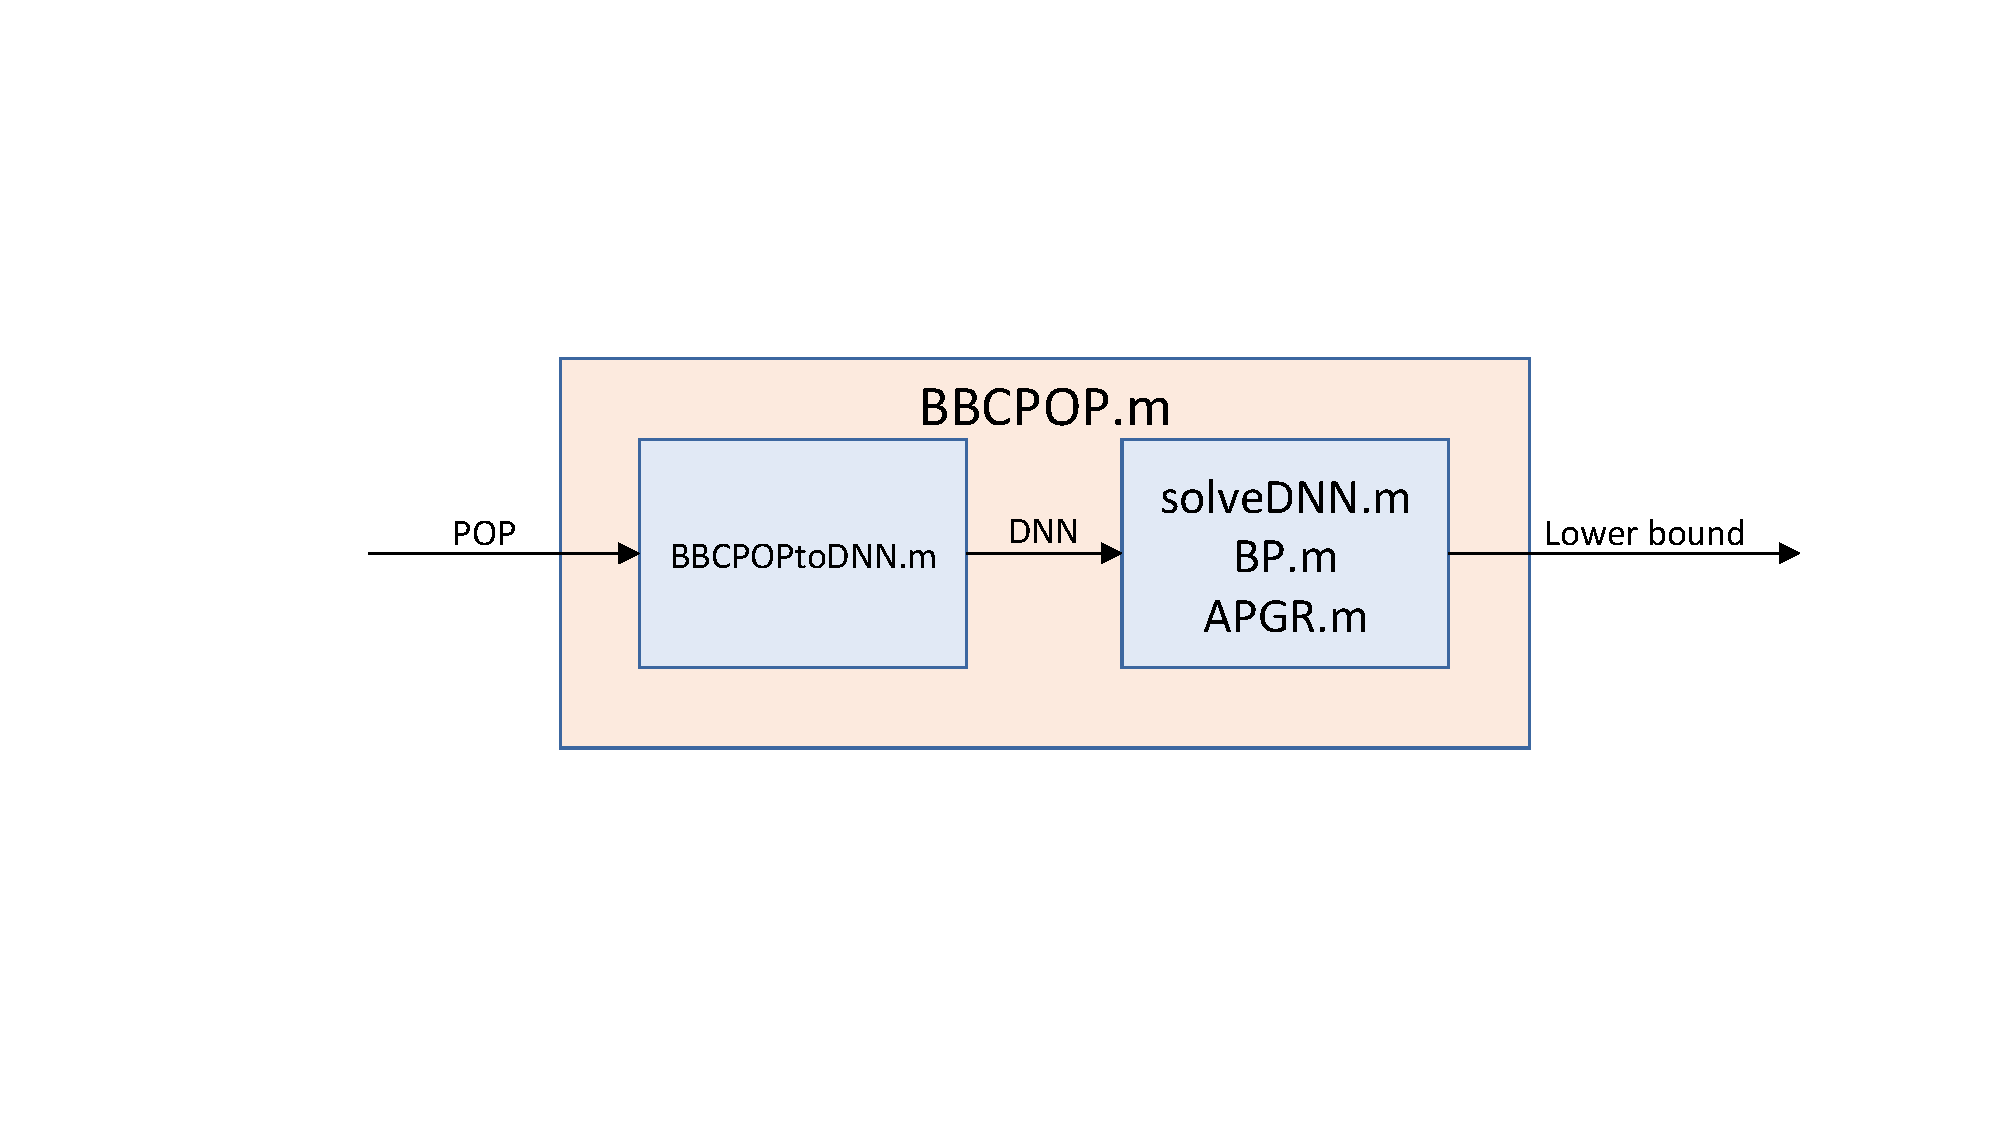
\includegraphics[width=13cm,height=5.cm]{BBCPOPstructure.pdf} 
\caption{The structure of the main function BBCPOP.m}
\end{center}
\end{figure}

Let $f_0$ be a real valued polynomial  defined on the $n$-dimensional Euclidean space $\Real^n$, 
$\Ibinary$ and $\Ibox$ a partition of $N\equiv\{1,2,\ldots,n\}$, {\it i.e.}, $\Ibinary\cup\Ibox = N$ and 
$\Ibinary\cap\Ibox=\emptyset$, and $\CC$ a family of subsets of $N$. 
Each POP in the class is described as
\begin{eqnarray}
\zeta^* & = & \min_{\x} \left\{ f_0(\x) \Big|
\begin{array}{l}
x_i\in\{0,1\} \ (i\in\Ibinary) \ \mbox{(box constraint)}, \\
x_j\in [0,1] \ (j\in\Ibox) \ \mbox{(binary constraint)}, \\
\displaystyle \prod_{j\in C} x_j = 0 \ (C \in \CC) \ \mbox{(complementarity constraint)} 
\end{array}
 \right\}. \label{eq:POP0} %\nonumber \\ 
%& = &   \min_{\x} \{ f_0(\x) \mid \x \in H \}, 
%  \label{eq:POP0} 
\end{eqnarray}

As an illustrative example, we consider the following POP with 
five variables $ x_1,x_2, x_3, x_4$ and $x_5$: 
 \begin{equation}
\left. 
 \begin{array}{ll}
	\mbox{minimize} & f_0(\x) \equiv 0.5x_1 -1.8x_3 -2.2x_5 +3x_3^2 +x_1x_2x_4 + 1.3x_2x_4x_5      \\
	\mbox{subject to} &  x_2x_3 = 0,\  x_3x_4 = 0, \  x_1, x_2 \in \{0,1\}, \  x_3, x_4, x_5 \in [0,1]  
	\end{array}
\right\} 
\label{ex:EX1}
\end{equation}
In this case, $\Ibinary = \{1,2\}$, $\Ibox = \{3,4,5\}$ and $\CC = \left\{ \{2,3\},\{3,4\} \right\}$.  
We can easily compute the optimal solution $\x^*=(0,0,0.3,0,1)$ and the optimal value $\zeta^*=-2.47$. 

The input of \matBP.m consists of the data for POP \eqref{eq:POP0}, the relaxation order $\omega$ which determines 
the hierarchy level of DNN relaxation to be constructed, and parameters which control the execution of 
\matBP.m. With the input data, \matBP.m constructs a simple conic optimization problem (COP):
\begin{eqnarray}
  y_0^* & = &  \max_{\scriptsize y_0,\Y_1, \Y_2}\{y_0 \mid  \Q_0 - y_0 \H_0 = \Y_1+ \Y_2, \ \Y_1 \in \coneK_1^*, 
\ \Y_2 \in \coneK_2^*\}
\label{eq:generalDualCOP0}, % \\
\end{eqnarray}
which serves as a DNN relaxation of POP~\eqref{eq:POP0} (hence $y_0^* \leq \zeta^*$). Here $\H_0$ denotes 
a constant vector in a linear space $\spaceV$ ($=$ the Cartesian product of symmetric matrix spaces) 
endowed with an inner product, % $\inprod{\cdot}{\cdot}$, 
$\coneK_1, \coneK_2 \subset \spaceV$ closed convex cones, and $y_0 \in\Real$, $\Y_1 \in \spaceV, \ \Y_2 \in \spaceV$ 
variables. The output of  \matBP.m is
 an approximate optimal solution $(y_0,\Y_1,\Y_2)$ of~\eqref{eq:generalDualCOP0} such that 
$y_0 \leq y_0^*$; hence $y_0 \leq \zeta^*$ is guaranteed. 

The degree of POP~\eqref{eq:POP0}  is defined as 
$ %\begin{eqnarray*}
\max\{ \mbox{deg}f_0, \ |C| \ (C \in \CC) \}, 
$ %\end{eqnarray*}
where $|C|$ denotes the number of elements in $C$ $(C \in \CC)$. 
The relaxation order $\omega$ needs to be a positive integer not less than 
the half of the degree of POP~\eqref{eq:POP0}. %\mbox{deg(POP\eqref{eq:POP0})}. 
Hence the minimum relaxation order that can be taken is  % given by 
\begin{eqnarray*}
\omega_{\min} = \mbox{the smallest positive integer not less than the half of the degree of POP~\eqref{eq:POP0}}. 
\end{eqnarray*} 
%In the case of POP~\eqref{ex:EX1}, $\omega_{\min}=2$. 
As we take a larger $\omega$, we can expect a tighter lower bound 
$y_0$ ($=$ the approximate optimal value of \eqref{eq:generalDualCOP0})  for $\zeta^*$, but 
COP~\eqref{eq:generalDualCOP0} to be solved by the BP Algorithm becomes larger, so that 
longer execution time is required. 
For many application problems in practice, taking $\omega_{\min}$ for the relaxation order $\omega$ is sufficient 
to obtain a tight lower bound for $\zeta^*$. 

In the above example~\eqref{ex:EX1}, we see that deg$f_0 = 3$, $|\{2,3\}| = 2$ and $|\{3,4\}| = 2$. 
Hence $\omega_{\min}= 2 \leq \omega$. 

In Section 2, we present how to describe POP \eqref{eq:POP0} for the input of the main function \matBP.m. In Section 3, 
we illustrate the execution of \matBP.m and present the details on the output of \matBP.m. Section 4 lists the parameters 
which control the execution of \matBP.m, and Section 5 some main functions contained in the \matBP\ software package.


\section{Representing polynomial optimization problems}

\label{Representation}

POP~\eqref{eq:POP0} is described by
\begin{eqnarray*}
{\sf objPoly}, \ {\sf I01} \ \mbox{ and } {\sf Icomp},
\end{eqnarray*}
which are input arguments of  \matBP.m. 
Let term$f_0$ denote the number of terms of $f_0$. 
We employ a simplified SparsePOP format to describe the objective function of POP~\eqref{eq:POP0}: 
\begin{center}
\begin{tabular}{rcll}
{\sf objPoly.supports}		& = & a set of supports of $f_0(\x)$, % \\
				% &	& & 
\ term$f_0$ $\times n$ matrix. \\
{\sf objPoly.coef}			& = & coefficients, % \\ 
				% &	& & a 
\ column vector of dimension term$f_0$. \\
\end{tabular}
\end{center}
For the original SparsePOP format, see \cite{SPARSEPOP_UG}. 
The functions simplifyPoly.m, 
addPoly.m and multiplyPoly.m in the directory polyTools/  can be used  % are useful to 
when describing an objective function $f_0(\x)$  % in the form of \eqref{POP2}
in the simplified SparsePOP format. 


The partition $\Ibinary\cup\Ibox$ of $N\equiv\{1,2,\ldots,n\}$ is described by the $n$-dimensional 
row vector  {\sf I01} such that 
\begin{eqnarray*}
 {\sf I01}_j = \left\{ \begin{array}{ll}
{\sf true}  & \mbox{if } j \in \Ibinary, \\ 
{\sf false} & \mbox{otherwise, {\it i.e.},  }  j \in \Ibox. 
\end{array} \right. 
\end{eqnarray*}
The family $\CC$ of subsets of $N$, which represents the complementarity condition in POP~\eqref{eq:POP0}, 
is represented by  {\sf Icomp}. Suppose that $\CC$ consists of $m$ nonempty subsets $C_1,\ldots,C_m$ of $N$. 
Then we set {\sf Icomp} to be the $m \times n$ matrix such that 
\begin{eqnarray*}
{\sf Icomp}_{ij} & = &
 \left\{ \begin{array}{ll}
{\sf true} & \mbox{if } j \in C_i, \\ 
{\sf false} & \mbox{otherwise, {\it i.e.},  }  j \not\in C_i
\end{array} \right. 
\end{eqnarray*}
$(i=1,\ldots,m, \ j=1,\ldots,n)$. If $\CC = \emptyset$, set ${\sf Icomp} = [\ ]$. 

The three input arguments {\sf objPoly},  {\sf I01} \ \mbox{ and } {\sf Icomp} for POP~\eqref{ex:EX1} 
are described as follows:
\begin{verbatim}
function [objPoly, I01, Icomp] = example1;
       objPoly.supports   = ...
                         [1 0 0 0 0;
                          0 0 1 0 0;
                          0 0 0 0 1;
                          0 0 2 0 0;
                          1 1 0 1 0;
                          0 1 0 1 1];
         objPoly.coef = [0.5; -1.8; -2.2; 3; 1; 1.3];	 
         Icomp = logical([0 1 1 0 0; 0 0 1 1 0]);
         I01 = logical([1 1 0 0 0]);
end 
\end{verbatim}

\section{Executing \matBP}

\label{sample}

A lower bound for the optimal value of POP~\eqref{ex:EX1} can be computed by \matBP.m\ as follows:
\begin{verbatim}
>>[objPoly, I01, Icomp] = example1;
>>relaxOrder = 2; params = [];
>>[sol, info] = BBCPOP(objPoly, I01, Icomp, relaxOrder, params);
\end{verbatim}

The following is shown on the screen  as the \matBP.m terminates at 17 iterations.



\begin{verbatim}
Original
iter=17:y0=-2.469903e+00,LBv=-2.470066e+00,[LB,UB]=[-2.470066e+00,-2.469903e+00]
Scaled
iter=17:y0=-9.058401e-01,LBv=-9.058999e-01,[LB,UB]=[-9.058999e-01,-9.058401e-01]

     LBv           y0            UB           UB-LBv   relnormX iter b_yes
 0  -1.000000e+21 +5.800000e+00 +5.800000e+00 9.80e+00 
 1  -4.536533e+01 +5.800000e+00 +5.800000e+00 9.80e+00 8.59e-01  101 90
 2  -1.867610e+01 +9.000000e-01 +9.000000e-01 4.90e+00 4.31e-01   56 1
 3  -6.974229e+00 -1.550000e+00 -1.550000e+00 2.45e+00 9.58e-02  218 90
 4  -2.775000e+00 -2.775000e+00 -1.550000e+00 1.22e+00 0.00e+00   17 2
 5  -2.775000e+00 -2.162500e+00 -2.162500e+00 6.12e-01 3.06e-02  301 88
 6  -2.476112e+00 -2.468750e+00 -2.162500e+00 3.14e-01 1.21e-04  350 88
 7  -2.476112e+00 -2.319306e+00 -2.319306e+00 1.57e-01 1.48e-02  274 90
 8  -2.476112e+00 -2.397709e+00 -2.397709e+00 7.84e-02 7.06e-03  180 90
 9  -2.476112e+00 -2.436911e+00 -2.436911e+00 3.92e-02 3.22e-03  301 88
10  -2.476112e+00 -2.456512e+00 -2.456512e+00 1.96e-02 1.31e-03  294 90
11  -2.476112e+00 -2.466312e+00 -2.466312e+00 9.80e-03 3.58e-04  301 88
12  -2.471212e+00 -2.471212e+00 -2.466312e+00 4.90e-03 0.00e+00   10 2
13  -2.471212e+00 -2.468762e+00 -2.468762e+00 2.45e-03 1.20e-04  301 88
14  -2.470066e+00 -2.469987e+00 -2.468762e+00 1.30e-03 1.29e-06  339 97
15  -2.470066e+00 -2.469414e+00 -2.469414e+00 6.52e-04 5.69e-05  339 97
16  -2.470066e+00 -2.469740e+00 -2.469740e+00 3.26e-04 2.53e-05  339 97
17  -2.470066e+00 -2.469903e+00 -2.469903e+00 1.63e-04 9.45e-06  301 99
 timeBP (Excecution time) = 1.98,  termcodeBP = 2
\end{verbatim}
The value  $ -2.470039e$+$00$ is the approximate optimal value of \eqref{ex:EX1} obtained by BP Algorithm, which is a valid lower bound 
of the optimal value $\zeta^* = -2.47$ of POP~\eqref{ex:EX1}. 

The output {\sf sol} is a structure containing the solution information for~\eqref{eq:generalDualCOP0}:
\begin{verbatim}
    y0init: 2.1272
       LBv: -2.4700
        LB: -2.4700
        UB: -2.4700
        Y1: [1×226 double]
        Y2: [1×226 double]
\end{verbatim}
Here {\sf y0init} corresponds to the initial value of $y_0^m$,  and   
{\sf LBv, LB, UB, Y1, Y2} to the terminal values of $y^{\ell v}_0$, $y^{\ell}$, $y^u_0$, 
$\hat{\Y}_1$ and $\hat{\Y}_2$, respectively,  in BP Algorithm in \cite{ITO2018}.
The output {\sf info} is a structure  
for some of the execution information of BP.m (BP Algorithm) and APGR.m 
(APGR Algorithm):
\begin{verbatim}
        iterBP: 17
        timeBP: 1.5884
    termcodeBP: 2
      iterAPGR: 3545
\end{verbatim}
Here {\sf iterBP} denotes the number of iteration of BP.m, {\sf timeBP} its execution time, 
{\sf termcodeBP} its termination code and {\sf iterAPGR} the total number of iterations of APGR.m. 
BP.m stops when 
\begin{description}
\item{(i) } the difference of the upper bound $y_0^u$ and the lower bound $y_0^\ell$ becomes 
 smaller than the prescribed parameter 
{\sf params.delta},
\item{(ii) } $(y_0^u-y_0^\ell)/\max\{1.0,|y_0^\ell|, |y_0^u|\}$ is smaller than the prescribed parameter
{\sf params.delta2}
\item{(iii) } the reduction of the length of the interval $[y_0^u-y_0^\ell]$ gets smaller than 
$\max\{{\sf params.delta},$ $ {\sf params.delta2}\}$.
\item{(iv) } the iteration of BP.m exceeds the prescribed parameter {\sf params.maxiterBP}, or 
\item{(v) } the execution time exceeds the prescribed parameter {\sf params.maxtimeBP}. 
\end{description}
These terminations are associated with the termination code 1,2,3,0,-1, respectively. 



\section{Parameters}
\label{PARAM}

In addition to {\sf objPoly}, {\sf I01}, {\sf Icomp} and {\sf relaxOrder} for  describing a POP,  
% in the SparsePOP format, 
the MATLAB function \matBP.m has {\sf params} as an input argument. It is a structure consisting of 
many parameters that control the performance of the function. Table \ref{tableOfparam} 
shows the list of parameters used in \matBP.m. The default values of parameters are given in the 
MATLAB function defaultParamBP.m. They can be modified if necessary. 

\begin{table}[htp]
\caption{The fields of {\sf params}, default values and possible values}
\begin{center}
\begin{tabular}{|l|l|l|} \hline
field of {\sf params} & default &  usage, possible values\\
\hline
\multicolumn{3}{|c|}{Parameters for DNN relaxation} \\ 
\hline 
{\sf sparseSW}   & 1 & Set 0 for dense DNN relaxation. \\
                           &    & Set 1 for sparse DNN relaxation. \\
\hline
\multicolumn{3}{|c|}{Parameters for BP and APGR Algorithms} \\ 
\hline
{\sf maxtimeBP }  & 20000 & the maximum execution time\\
\hline
{\sf maxiterBP} & 40 & the maximum iteration  for BP Algorithm \\
\hline
{\sf maxiterAPGR}  & 20000 & the maximum iteration for APGR Algorithm \\
\hline
{\sf delta1}  & 1e-4 & the relative tolerance for BP Algorithm\\
                             &    & Set $0$ if {\sf delta} is used. \\
\hline
{\sf delta}  & 0 & the absolute tolerance  for BP Algorithm \\
                         &    & Set  ${\sf delta} \in (0,1)$ if $\zeta^*$ is integer. \\
                         &    & Set $0$ otherwise. \\
\hline
{\sf printyes}  & 2 & print level, 0,1,2 or 3 \\  
\hline                        
{\sf UbdObjVal}   & $f_0(\0)$   & the upper bound %\\
%                  &             & 
for the optimal value $\zeta^*$ of POP~\eqref{eq:POP0} \\
\hline
{\sf UbdIX}          &         & $= \rho$ given in Assumption (A1) of \cite{ITO2018}.\\
                     &         & To specify this parameter, see Sections 2.3 and 4.1 of \cite{ITO2018}. \\
\hline
\end{tabular}
\end{center}
\label{tableOfparam}
\end{table}


%% Skim 5/15/07
\section{Description of main and principal subfunctions}
%The main MATLAB functions and important subfunctions}
\label{mainFunctions}

The main function and principal subfunctions are described in terms of input and output
arguments in this section. 

\subsection{The MATLAB functions sparsePOP.m, SDPrelaxation.m, and SDPrelaxationMex.m} 


The main function sparsePOP.m, its principal subfunctions SDPrelaxation.m 
% Skim 5/15/07
and SDPrelaxationMex.m  shown in Figure~\ref{structure} 
have the following function declarations: 
\begin{verbatim}
function [param,SDPobjValue,POP,cpuTime,SeDuMiInfo,SDPinfo] = ...
    sparsePOP(objPoly,ineqPolySys,lbd,ubd,param); 

function [param,SDPobjValue,POP,cpuTime,SeDuMiInfo,SDPinfo] = ...
    SDPrelaxation(param,objPoly,ineqPolySys,lbd,ubd);

function [param,SDPobjValue,POP,cpuTime,SeDuMiInfo,SDPinfo] = ...
    SDPrelaxationMex(param,objPoly,ineqPolySys,lbd,ubd);
\end{verbatim}
respectively. These three functions have the same input and output 
arguments. Among the input arguments, {\sf param} contains a set of parameters
% Skim 5/15/07 
% Kojima 5/18/07 
% for choosing certain algorithmic procedures. % their behavior.
% More 
whose detailed description is included in Section \ref{PARAM}. 
The other input arguments, if all of them are specified,   describe a POP 
in the SparsePOP format, as presented in Section~4.2. 

Although sparsePOP.m is defined with 5 input arguments, using 1 or 2 input arguments
is also possible as mentioned in Section~\ref{sample}. 
%the following usages with 1 or 2 input arguments are also possible: 
\begin{itemize}
\item ${\bf >>}$ {\sf sparsePOP('example1.gms')} for solving a POP described in the GAMS scalar format 
with the default {\sf param}. 
\item ${\bf >>}$ {\sf sparsePOP('example1.gms',param)} for solving a POP described in the GAMS scalar 
format with the user-specified {\sf param}. 
\item ${\bf >>}$ {\sf sparsePOP('example1')} for solving a POP described in the SparsePOP  format with 
the default {\sf param}. 
\item ${\bf >>}$ {\sf sparsePOP('example1',param)} for solving a POP described in the SparsePOP format 
with the user-specified {\sf param}. 
\end{itemize}
%These have been illustrated in Section~\ref{sample}. 

If the SDPrelaxation.m or the SDPrelaxationMex.m is to be utilized directly,
%On the other hand,
 either a set of the 5 input arguments 
\[
\mbox{ {\sf param}, {\sf objPoly}, {\sf ineqPolySys}, {\sf lbd} and {\sf ubd} } 
\]
or a set of the 3 input arguments 
\[
\mbox{ {\sf param}, {\sf objPoly} and {\sf ineqPolySys}} 
\]
needs to be specified. %if the user utilize the sparsePOPmain.m or the sparsePOPmainMex.m directly. 
%In the latter  3 input arguments case, 
In the case that 3 input arguments are prescribed,
the functions SDPrelaxation.m and SDPrelaxationMex.m assign the default values 
% Skim 5/24/07
{\sf lbd}$(i) = -1.0$e+$10$ and  {\sf ubd}$(i) = +1.0$e+$10$ $(i=1,2,\ldots,n)$, which implies that 
$-\infty < x_i < \infty$ $(i=1,2,\ldots,n)$.  

For the output arguments, user-specified or default values for the parameters are stored  in {\sf param}.
{\sf SDPobjValue} contains a lower bound for the optimal objective value of the POP (\ref{POP0}). 
% Skim 5/15/07
\mbox{For every feasible solution $\x$ of the POP (\ref{POP0})},
\begin{eqnarray}
\mbox{{\sf SDPobjValue}}  \leq f_0(\x) \label{lowerBound} 
\end{eqnarray}
holds. %\mbox{for every feasible solution $\x$ of (\ref{POP0})}. 
The output argument {\sf POP} has four components: 
\begin{itemize}
\item {\sf POP.xVect}: a candidate $\x^{\omega}$ of an optimal solution of  the POP (\ref{POP0}). 
\item {\sf POP.objValue}: 
the objective function value $f_0(\x^{\omega})$ at $\x^{\omega} = $ {\sf POP.xVect}.
\item {\sf POP.absError}: an  absolute feasibility error at  $\x^{\omega}$. 
\item {\sf POP.scaledError}: a scaled feasibility error $\x^{\omega}$. 
\end{itemize}
(Recall that the relaxation order $\omega = $ {\sf param.relaxOrder} determines the 
quality of the SDP relaxation of the POP). % to be solved). 
Here the absolute feasibility error 
at $\x^{\omega}$ is given by 
\begin{eqnarray*}
\min \left\{ \min\{ f_i(\x^{\omega}), \ 0 \} \ (i=1,2,\ldots,\ell), \ - |f_j(\x^{\omega})| \ (j=\ell+1,\ldots,m) \right\}, 
\end{eqnarray*}
and the scaled feasibility error  
is given by 
\begin{eqnarray*}
\min \left\{ \min\{ f_i(\x^{\omega})/\sigma_i(\x^{\omega}), \ 0 \} \ (i=1,2,\ldots,\ell), \ - |f_j(\x^{\omega})|/\sigma_j(\x^{\omega}) \ (j=\ell+1,\ldots,m) \right\}, 
\end{eqnarray*}
where $\sigma_i(\x^{\omega})$ denotes the maximum of the absolute values 
of all monomials 
of $f_i(\x)$ evaluated at $\x^{\omega}$ if the maximum is greater than $1$, 
or $\sigma_i(\x^{\omega}) = 1$ otherwise $(i=1,2,\ldots,m)$. 
Note that both errors are always nonpositive. 
The relative error in the objective value at $\x^{\omega}$ in the output of sparsePOP.m, 
which has been illustrated in Section 4,  is computed as 
\[
\mbox{{\sf   relative obj error}} = \frac{{\sf POP.objValue} - {\sf SDPobjValue}}{\max \{ 1, |{\sf POP.objValue}| \}}. 
\]
If {\sf POP.scaledError} $\leq 0$ is close to $0$, say $-1.0$e-$6 \leq $  {\sf POP.scaledError} $\leq 0$, 
we may regard that $\x^{\omega}$ is feasible approximately. If, in addition, 
{\sf   relative obj error} $ \geq 0$ is close to $0$, say $0 \leq $ {\sf   relative obj error} $\leq 1.0$e-$6$, 
% Skim 5/15/07 provides
$\x^{\omega}$ is an approximate optimal solution of the POP (\ref{POP0}). 

The output argument {\sf cpuTime} shows various cpu times consumed by 
% Skim 5/24/07
%the execution of
 sparsePOP.m:
\begin{itemize}
\item  {\sf cpuTime.conversion}: 
the cpu time consumed to convert the POP into its SDP relaxation. 
\item {\sf cpuTime.SeDuMi}: the cpu time consumed by SeDuMi to solve the SDP.
\item {\sf cpuTime.Total}: the cpu time for the entire process.
\end{itemize}

The output argument {\sf SDPinfo} has information of the SDP relaxation problem solved 
by SeDuMi.
\begin{itemize}
\item {\sf SDPinfo.rowSizeA}:
the number of rows  of the coefficient matrix $\A$ of the SDP.  
\item {\sf SDPinfo.colSizeA}:
the number of  columns of the coefficient matrix $\A$. % of the primal SDP 
\item {\sf SDPinfo.nonzeroInA}: the number of nonzeros of the 
coefficient matrix $A$.
\item {\sf SDPinfo.noOfLPvariables}:
the number of LP variables of the SDP.
\item {\sf SDPinfo.noOfFRvariables}: the number of free variables of the SDP. 
\item {\sf   SDPinfo.SDPblock}:
the row vector of the sizes of SDP blocks.
\end{itemize}

Finally, the output argument 
{\sf SeDuMiInfo} contains {\sf SeDuMiInfo.numerr}, {\sf SeDuMiInfo.pinf},
and {\sf SeDuMi.dinf}, which
are equivalent to info.numerr, info.pinf, and info.dinf in SeDuMi output.
See \cite{STRUM99} for the details.

\subsection{The MATLAB function readGMS.m} 

The MATLAB function readGMS.m has the following function declaration:
\begin{verbatim}
function [objPoly,ineqPolySys,lbd,ubd] = readGMS(fileName,symbolicMath);
\end{verbatim}
% Skim 5/15/07
The first argument {\sf fileName}, a string in MATLAB,
is the name of the file where a problem is described
in the \GMS format. It must have the extension .gms such as 'example1.gms'. 
The second input argument {\sf symbolicMath} is set to be $1$ by default, assuming that 
the Symbolic Math Tool is available. It should be set to $0$ if it is not available. 
The output of {\sf objPoly}, {\sf ineqPolySys}, {\sf lbd}, and {\sf ubd} 
is a POP data in  the SparsePOP format, and can be passed to SDPrelaxation.m
or SDPrelaxationMex.m.


\subsection{The MATLAB function printSolution.m} 

The function printSolution.m for printing the results has
the following function declaration.
\begin{verbatim}
function printSolution(fileId,printLevel,dataFileName,param,SDPobjValue,...
        POP,cpuTime,SeDuMiInfo,SDPinfo);
\end{verbatim}
The meaning of each input argument is as follows.
\begin{itemize}
\item {\sf fileId}: fileId where output is printed. If fileId is $1$,
then the result is displayed on the screen (i.e., the standard output).
If the result in a file is desired,
% Skim 5/15/07 
the file should be open in writable mode before specifying it in fileId.
\item {\sf printLevel}: a larger value of printLevel gives more detailed description
of the result. Default is $2$.
\item {\sf dataFileName}: the name of the problem solved.
\end{itemize}
The rest of the input arguments, i.e.,
{\sf param},
{\sf SDPobjValue},
{\sf POP},
{\sf cpuTime},
{\sf SeDuMiInfo}, and 
{\sf SDPinfo} should be the output of 
SDPrelaxation.m and SDPrelaxationMex.m.




\section{Some functions}

\label{mainFunctions}

We list some functions contained in the \matBP\ software package. Important subfunctions 
of \matBP.m are listed in 
Section~5.1, and functions for some test instances are listed in Section~5.2. 

\subsection{Main subfunctions of \matBP.m}



\begin{description}
\item{relaxation/BBCPOPtoDNN.m} constructs COP~\eqref{eq:generalDualCOP0}, 
which serves as a DNN relaxation of~\eqref{eq:POP0}. 
\item{solver/solveDNN.m } solves COP~\eqref{eq:generalDualCOP0} by applying BP Algorithm and APGR Algorithm.
\item{solver/BP/BP.m } is an implementation of BP Algorithm in \cite{ITO2018}.
\item{solver/BP/APGR.m} is an implementation of APGR Algorithm in \cite{ITO2018}.
\end{description}

\subsection{Functions for POP instances}

All the functions below output {\sf objPoly}, {\sf I01}, {\sf Icomp}, {\sf relaxOrder} $=\omega_{min}$ and {\sf params}, which 
can be used as input of \matBP.m.
\begin{description}
\item{instances/POPrandom/genPOPdense.m } generates a dense POP instance with binary, box and complementarity constraints.
\begin{verbatim}
>> degree=3; nDim=5; isBin=true; addComplement=false; 
>> [objPoly,I01,Icomp,relaxOrder,params] = ... 
        genPOPdense(degree,nDim,isBin,addComplement); 
\end{verbatim}
\item{instances/POPrandom/genPOParrow.m } generates a sparse POP instance (whose objective function $f_0(\x)$ has 
an arrow type sparsity pattern Hessian matrix) with binary, box and complementarity constraints.
\begin{verbatim}
>> degree=4; a=10; b=2; c=2; l=3; isBin=0; addComplement=true; 
>> [objPoly, I01, Icomp, relaxOrder, params] = ...
        genPOParrow(degree,a,b,c,l,isBin,addComplement);
\end{verbatim}
\item{instances/POPrandom/genPOPchordal.m } generates a sparse POP instance (whose objective function $f_0(\x)$ has 
a sparse Hessian matrix characterized by a chordal graph) with binary, box and complementarity constraints.
\begin{verbatim}
>> degree=3; nDim=100; radiorange=0.1; isBin=1; addComplement=false;
>> [objPoly, I01, Icomp, relaxOrder, params] = ...
        genPOPchordal(degree,nDim,radiorange,isBin,addComplement);
\end{verbatim}
\item{instances/QAP/qapreadBP.m} generates a QOP with box and complementarity constraints which is induced from a Lagrangian relaxation of a QAP instance from QAPLIB \cite{QAPLIB}.
\begin{verbatim}
>> instance='chr12a'; lambda=10000; 
>> [objPoly, Icomp, I01, relaxOrder, params] = ...
        qapreadBP(instance,lambda);
\end{verbatim}
\item{instances/BIQ/biqreadBP.m} generates a QOP with box and complementarity constraints which is induced from a Lagrangian 
relaxation of a binary/box constrained QOP instance from  BIQMAC \cite{BIQMAC}.
\begin{verbatim}
>> instance='bqp100-1'; lambda=10000;
>> [objPoly, I01, Icomp, relaxOrder, params] = ...
        biqreadBP(instance,lambda);
\end{verbatim}
\end{description}




\bibliographystyle{plain}


\begin{thebibliography}{1}

\bibitem{ARIMA2017}
N.~Arima, S.~Kim, M.~Kojima, and K.C. Toh.
\newblock A robust \mbox{Lagrangian-DNN} method for a class of quadratic
  optimization problems.
\newblock {\em Comput. Optim. Appl.}, 66(3):453--479, 2017.

\bibitem{BECK2009}
A.~Beck and M.~Teboulle.
\newblock A fast iterative shrinkage-thresholding algorithm for linear inverse
  problems.
\newblock {\em SIAM J. Imaging Sci.}, 2:183--202, 2009.

\bibitem{QAPLIB}
P.~Hahn and M.~Anjos.
\newblock {QAPLIB} -- a quadratic assignment problem library.
\newblock http://www.seas.upenn.edu/qaplib.

\bibitem{ITO2018}
N.~Ito, S.~Kim, M.~Kojima, A.~Takeda, and K.~C. Toh.
\newblock {BBCPOP}: {A} sparse doubly nonnegative relaxation of {P}olynomial
  {O}ptimization {P}roblems with {B}inary, {B}ox and {C}omplementarity
  constraints.
\newblock Research {R}port {B}-48?, {T}okyo {I}nstitute of {T}echnology,
  {D}epartment of {M}athematical and {C}omputing {S}ciences, {T}okyo
  {I}nstitute of {T}echnology, {O}h-{O}kayama, {M}eguro-ku, {T}okyo 152-8552,
  March 2018.

\bibitem{KIM2016}
S.~Kim, M.~Kojima, and K.~C. Toh.
\newblock Doubly nonnegative relaxations for quadratic and polynomial
  optimization problems with binary and box constraints.
\newblock Research {R}port {B}-483, {T}okyo {I}nstitute of {T}echnology,
  {D}epartment of {M}athematical and {C}omputing {S}ciences, {O}h-{O}kayama,
  {M}eguro-ku, T{}okyo 152-8552, July 2016.

\bibitem{KIM2013}
S.~Kim, M.~Kojima, and K.~C. Toh.
\newblock A {L}agrangian-{DNN} relaxation: a fast method for computing tight
  lower bounds for a class of quadratic optimization problems.
\newblock {\em Math. {P}rogram.}, 156:161--187, 2016.

\bibitem{SPARSEPOP_UG}
H.~Waki, S.~Kim, M.~Kojima, M.~Muramatsu, H.~Sugimoto, and M.~Yamashita.
\newblock {\em User Manual for SparsePOP: a Sparse Semidefinite Programming
  Relaxation of Polynomial Optimization Problems}.
\newblock https://sourceforge.net/projects/sparsepop/?source={typ\_redirect},
  August 2009.

\bibitem{BIQMAC}
A.~Wiegele.
\newblock Biq mac library.
\newblock http://www.biqmac.uni-klu.ac.at/biqmaclib.html, 2007.

\end{thebibliography}



\end{document}

